\documentclass{beamer}
\usepackage{tikz}
\usetikzlibrary{positioning}
\usepackage{graphicx}
\usetheme{CambridgeUS}
\usepackage{xcolor, bm}  

\definecolor{myred}{RGB}{139,0,0}  
\setbeamercolor{palette primary}{bg=myred, fg=white}

% Footer and Header Customization
\setbeamertemplate{headline}{%
    \leavevmode%
    \hbox{%
        \begin{beamercolorbox}[wd=\paperwidth, ht=0.4cm, dp=0cm, left]{palette primary}%
        \end{beamercolorbox}%
    }%
}
\setbeamertemplate{footline}
{
  \leavevmode
  \hbox{
    \begin{beamercolorbox}[wd=.3\paperwidth,ht=2.5ex,dp=1.125ex,left]{author in head/foot}
      \hspace{.5cm} bscs23074 \& bscs23198 (ITU)
    \end{beamercolorbox}%
    \begin{beamercolorbox}[wd=.4\paperwidth,ht=2.5ex,dp=1.125ex,center]{title in head/foot}
      Algorithms, Design \& Analysis
    \end{beamercolorbox}%
    \begin{beamercolorbox}[wd=.3\paperwidth,ht=2.5ex,dp=1.125ex,right]{date in head/foot}
      \insertframenumber / \inserttotalframenumber \hspace{.5cm}
    \end{beamercolorbox}%
  }
  \vskippt
}
\title{Algorithms, Design \& Analysis}
\subtitle{Lecture 17: Single Source Shortest Path}
\author{Ifra Abdul Rauf \& Mishaal Mustazhar}
\institute{Information Technology University}
\date{March 25, 2025}
\logo{
\includegraphics[height=1cm]{university_logo}}  

% slides ============

\begin{document}

    \begin{frame}
        \setbeamercolor{title}{bg=myred, fg = white}
        \setbeamercolor{subtitle}{fg=white}
        \titlepage
    \end{frame}
    
    \begin{frame}
        \frametitle{About Your Fellows}
        \begin{itemize}
            \item Hi there! We are \textcolor{red}{\textbf{Ifra}} {and }\textcolor{red}{\textbf{Mishaal}}.
            \item We are Associate Students at ITU.
        \end{itemize}
    \end{frame}
    
    \begin{frame}{Single Source Shortest Path}
        \begin{itemize}
            \item For \textbf{weighted}, \textbf{directed} graphs.
            \item \textbf{\textcolor{blue}{Goal}} : Find the \textcolor{red}{shortest path} from a single source node to all other nodes while considering edge weights.
        \end{itemize}
    \end{frame}
    
    \begin{frame}{Applications}
        \textbf{Navigation Systems (e.g., Google Maps, GPS)}
        \begin{itemize}
            \item Computes the fastest or shortest route from a given location to multiple destinations.
            \item Considers road distances, traffic conditions, and time.
        \end{itemize}
        \textbf{Airline Route Optimization}
        \begin{itemize}
            \item Determines the most efficient flight paths between airports.
            \item Reduces fuel costs and optimizes travel time based on available routes.
        \end{itemize}
    \end{frame}
    
    \begin{frame}{Example Graph}
        \centering
        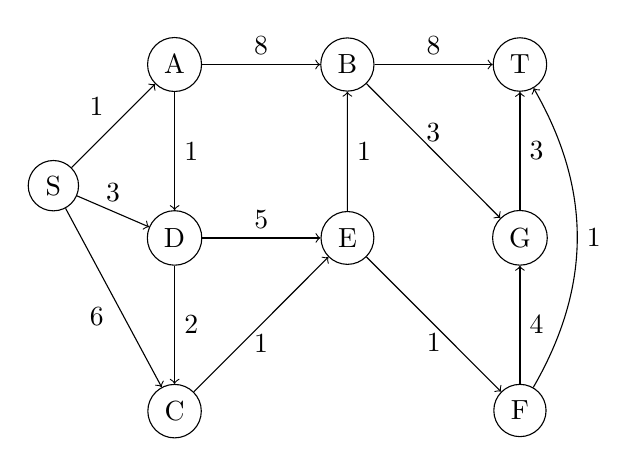
\begin{tikzpicture}[node distance=15mm, main/.style = {draw, circle}] 
                
            % Nodes
            \node[main] (S) {S};
            \node[main] (A) [above right=of S] {A};
            \node[main] (B) [right=of A] {B};
            \node[main] (D) [below=of A] {D};
            \node[main] (C) [below=of D] {C};
            \node[main] (E) [right=of D] {E};
            \node[main] (T) [right=of B] {T};
            \node[main] (G) [below =of T] {G};
            \node[main] (F) [below =of G] {F};
        
            % Edges with weights
            \draw[->] (S) --  node[midway, above left] {1} (A);
            \draw[->] (S) --  node[midway, above] {3} (D);
            \draw[->] (S) --  node[midway, below left] {6} (C);
            \draw[->] (A) --  node[midway, above] {8} (B);
            \draw[->] (A) --  node[midway, right] {1} (D);
            \draw[->] (D) --  node[midway, above] {5} (E);
            \draw[->] (D) --  node[midway, right] {2} (C);
            \draw[->] (C) --  node[midway, below] {1} (E);
            \draw[->] (B) --  node[midway, above] {8} (T);
            \draw[->] (B) --  node[midway, above] {3} (G);
            \draw[->] (E) --  node[midway, below] {1} (F);
            \draw[->] (E) --  node[midway, right] {1} (B);
            \draw[->] (F) --  node[midway, right] {4} (G);
            \draw[->] (G) --  node[midway, right] {3} (T);
            
            % Curved Edge from F to T
            \draw[->, bend right=30] (F) to node[midway, right] {1} (T);
        \end{tikzpicture}
    
        \vspace{1em}
    \end{frame}
        \newpage 
    
    \begin{frame}{paths from S to T}
            Let’s consider multiple paths from \textbf{S} to \textbf{T}
    \end{frame}
        
    \begin{frame}{Path 1}
        \textbf{One possible path is:}
        
        \begin{center}
            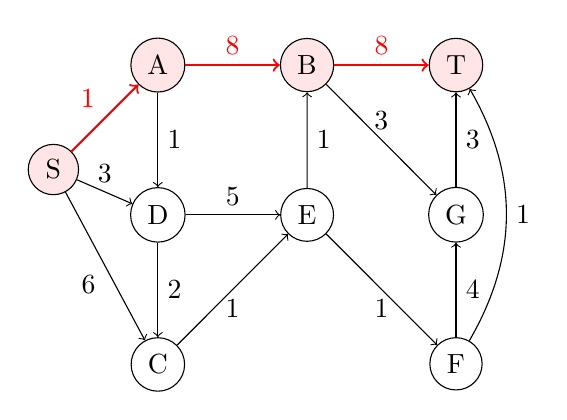
\begin{tikzpicture}[node distance=12mm, main/.style = {draw, circle}] 
                    
                % Nodes
                \node[main,fill=red!10] (S) {S};
                \node[main,fill=red!10] (A) [above right=of S] {A};
                \node[main,fill=red!10] (B) [right=of A] {B};
                \node[main] (D) [below=of A] {D};
                \node[main] (C) [below=of D] {C};
                \node[main] (E) [right=of D] {E};
                \node[main,fill=red!10] (T) [right=of B] {T};
                \node[main] (G) [below =of T] {G};
                \node[main] (F) [below =of G] {F};
            
                % Edges with weights
                \draw[->, thick, red] (S) --  node[midway, above left] {1} (A);
                \draw[->] (S) --  node[midway, above] {3} (D);
                \draw[->] (S) --  node[midway, below left] {6} (C);
                \draw[->, thick, red] (A) --  node[midway, above] {8} (B);
                \draw[->] (A) --  node[midway, right] {1} (D);
                \draw[->] (D) --  node[midway, above] {5} (E);
                \draw[->] (D) --  node[midway, right] {2} (C);
                \draw[->] (C) --  node[midway, below] {1} (E);
                \draw[->, thick, red] (B) --  node[midway, above] {8} (T);
                \draw[->] (B) --  node[midway, above] {3} (G);
                \draw[->] (E) --  node[midway, below] {1} (F);
                \draw[->] (E) --  node[midway, right] {1} (B);
                \draw[->] (F) --  node[midway, right] {4} (G);
                \draw[->] (G) --  node[midway, right] {3} (T);
                % Curved Edge from F to T
                \draw[->, bend right=30] (F) to node[midway, right] {1} (T);
            
            \end{tikzpicture}
        \end{center} 
        
        \textbf{Path:} $S \rightarrow A \rightarrow B \rightarrow T$ \\ 
        \textbf{Cost:} $1 + 8 + 8 = 17$
        
    \end{frame}
    
    
    \begin{frame}{Path 2}
        \textbf{Another possible path is:}
        
        \begin{center}
            \begin{tikzpicture}[node distance=12mm, main/.style = {draw, circle}]                
                % Nodes
                \node[main,fill=red!10] (S) {S};
                \node[main,fill=red!10] (A) [above right=of S] {A};
                \node[main] (B) [right=of A] {B};
                \node[main,fill=red!10] (D) [below=of A] {D};
                \node[main,fill=red!10] (C) [below=of D] {C};
                \node[main,fill=red!10] (E) [right=of D] {E};
                \node[main,fill=red!10] (T) [right=of B] {T};
                \node[main] (G) [below =of T] {G};
                \node[main,fill=red!10] (F) [below =of G] {F};
            
                % Edges with weights
                \draw[->, thick, red] (S) --  node[midway, above left] {1} (A);
                \draw[->] (S) --  node[midway, above] {3} (D);
                \draw[->] (S) --  node[midway, below left] {6} (C);
                \draw[->] (A) --  node[midway, above] {8} (B);
                \draw[->, thick, red] (A) --  node[midway, right] {1} (D);
                \draw[->] (D) --  node[midway, above] {5} (E);
                \draw[->, thick, red] (D) --  node[midway, right] {2} (C);
                \draw[->, thick, red] (C) --  node[midway, below] {1} (E);
                \draw[->] (B) --  node[midway, above] {8} (T);
                \draw[->] (B) --  node[midway, above] {3} (G);
                \draw[->, thick, red] (E) --  node[midway, below] {1} (F);
                \draw[->] (E) --  node[midway, right] {1} (B);
                \draw[->] (F) --  node[midway, right] {4} (G);
                \draw[->] (G) --  node[midway, right] {3} (T);
                % Curved Edge from F to T
                \draw[->, bend right=30, thick, red] (F) to node[midway, right] {1} (T)  
                
            \end{tikzpicture}
        \end{center} 
        
        \textbf{Path:} $S \rightarrow A \rightarrow D \rightarrow C \rightarrow E \rightarrow F \rightarrow T$ \\
        \textbf{Cost:} $1 + 1 + 2 + 1 + 1 + 1 = 7$. \\
    \end{frame}


    \begin{frame}{Path Comparison}
        \centering
        \textcolor{red}{\textbf{Comparison of paths}} \\ % Text above
        \\
        \begin{minipage}{0.45\textwidth}
            \textbf{Path 1:} \\[0.5ex]  % Ensures space between text and graph
            \centering
             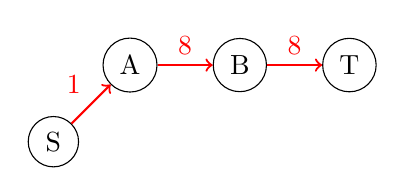
\begin{tikzpicture}[node distance=7mm, main/.style = {draw, circle}] 
                
            % Nodes
            \node[main] (S) {S};
            \node[main] (A) [above right=of S] {A};
            \node[main] (B) [right=of A] {B};
            \node[main] (T) [right=of B] {T};
        
            % Edges with weights
            \draw[->, thick, red] (S) --  node[midway, above left] {1} (A);
            \draw[->, thick, red] (A) --  node[midway, above] {8} (B); 
            \draw[->, thick, red] (B) --  node[midway, above] {8} (T);

        \end{tikzpicture}  \\[1ex]
            \textit{\textbf{Cost:}} $1 + 8 + 8 = 17$
        \end{minipage}
        \hfill
        \begin{minipage}{0.45\textwidth}
        \vspace{4ex}  % Adjust this to align Path 2 text properly
        \textbf{Path 2:}  
        \begin{center}
            \begin{tikzpicture}[node distance=6mm, main/.style = {draw, circle}]   
                % Nodes
                \node[main] (S) {S};
                \node[main] (A) [above right=of S] {A}; 
                \node[main] (D) [below=of A] {D};
                \node[main] (C) [below=of D] {C};
                \node[main] (E) [ right=of D] {E};
                \node[main] (T) [right=of B] {T}; 
                \node[main] (F) [below right=of E] {F};
            
                % Edges with weights
                \draw[->, thick, red] (S) --  node[midway, above left] {1} (A); 
                \draw[->, thick, red] (A) --  node[midway, right] {1} (D); 
                \draw[->, thick, red] (D) --  node[midway, right] {2} (C);
                \draw[->, thick, red] (C) --  node[midway, below] {1} (E); 
                \draw[->, thick, red] (E) --  node[midway, below] {1} (F);
                % Curved Edge from F to T
                \draw[->, bend right=30, thick, red] (F) to node[midway, right] {1} (T)  
                
            \end{tikzpicture}
    \end{center}  \\[1ex]
            \textit{\textbf{Cost:}} $1 + 1 + 2 + 1 + 1 + 1 = 7$. \\
        \end{minipage}
    
        % \vspace{0.1cm}
        \textbf{Observation:} path 2 has more edges, but less cost.
    \end{frame}
    
    \begin{frame}{How to Find the Shortest Path?}
        
        \textbf{Naive Approach:}
        \begin{itemize}
            \item List all possible paths from the source to the destination.
            \item Calculate the total weight for each path.
            \item Choose the one with the minimum weight.
        \end{itemize}
        
    \end{frame}
    
    % Slide 4: Why Brute Force Fails
    \begin{frame}{Why Brute Force Doesn't Work?}

        What happens in graphs with \textbf{multiple decision points}? \\ 
        Consider the following example:
         
        \begin{center}

            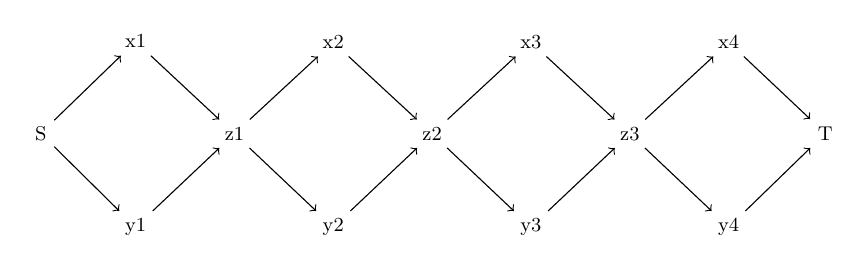
\begin{tikzpicture}[scale=0.8, transform shape] 
                \tikzstyle{main}=[font=\small]
                    
                % Nodes
                \node[main] (S) {S};
                
                \node[main] (x1) [above right=of S] {x1};
                \node[main] (y1) [below right=of S] {y1};
                \node[main] (z1) [above right=of y1] {z1};
        
                \node[main] (x2) [above right=of z1] {x2};
                \node[main] (y2) [below right=of z1] {y2};
                \node[main] (z2) [above right=of y2] {z2};
        
                \node[main] (x3) [above right=of z2] {x3};
                \node[main] (y3) [below right=of z2] {y3};
                \node[main] (z3) [above right=of y3] {z3};
        
                \node[main] (x4) [above right=of z3] {x4};
                \node[main] (y4) [below right=of z3] {y4};
                \node[main] (T) [above right=of y4] {T};
        
                % % Edges with weights
                \draw[->] (S)  -- (x1);
                \draw[->] (S)  -- (y1);
                \draw[->] (x1) -- (z1);
                \draw[->] (y1) -- (z1);
        
                \draw[->] (z1) -- (x2);
                \draw[->] (z1) -- (y2);
                \draw[->] (x2) -- (z2);
                \draw[->] (y2) -- (z2);
        
                \draw[->] (z2) -- (x3);
                \draw[->] (z2) -- (y3);
                \draw[->] (x3) -- (z3);
                \draw[->] (y3) -- (z3);
                
                \draw[->] (z3) -- (x4);
                \draw[->] (z3) -- (y4);
                \draw[->] (x4) -- (T);
                \draw[->] (y4) -- (T);
                
            \end{tikzpicture}
        \end{center}
    
        \centering
        
    \end{frame}
    
    
    \begin{frame}{Decision Paths and Their Growth}
        
        \begin{center}
            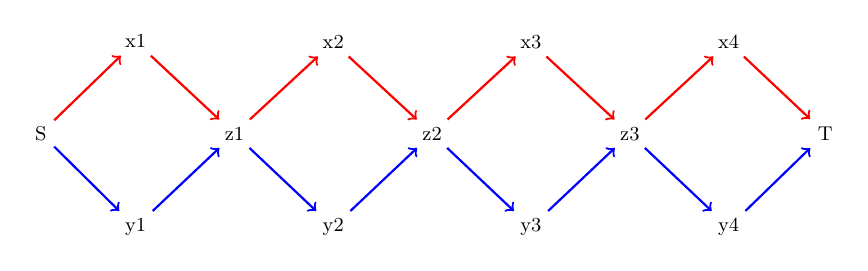
\begin{tikzpicture}[scale=0.8, transform shape] 
                \tikzstyle{main}=[font=\small]
                % Nodes
                \node[main] (S) {S};
                
                \node[main] (x1) [above right=of S] {x1};
                \node[main] (y1) [below right=of S] {y1};
                \node[main] (z1) [above right=of y1] {z1};
        
                \node[main] (x2) [above right=of z1] {x2};
                \node[main] (y2) [below right=of z1] {y2};
                \node[main] (z2) [above right=of y2] {z2};
        
                \node[main] (x3) [above right=of z2] {x3};
                \node[main] (y3) [below right=of z2] {y3};
                \node[main] (z3) [above right=of y3] {z3};
        
                \node[main] (x4) [above right=of z3] {x4};
                \node[main] (y4) [below right=of z3] {y4};
                \node[main] (T) [above right=of y4] {T};
        
                % % Edges with weights
                \draw[->,thick, red] (S)  -- (x1);
                \draw[->,thick, blue] (S)  -- (y1);
                \draw[->,thick, red] (x1) -- (z1);
                \draw[->,thick, blue] (y1) -- (z1);
        
                \draw[->,thick, red] (z1) -- (x2);
                \draw[->,thick, blue] (z1) -- (y2);
                \draw[->,thick, red] (x2) -- (z2);
                \draw[->,thick, blue] (y2) -- (z2);
        
                \draw[->,thick, red] (z2) -- (x3);
                \draw[->,thick, blue] (z2) -- (y3);
                \draw[->,thick, red] (x3) -- (z3);
                \draw[->,thick, blue] (y3) -- (z3);
                
                \draw[->,thick, red] (z3) -- (x4);
                \draw[->,thick, blue] (z3) -- (y4);
                \draw[->,thick, red] (x4) -- (T);
                \draw[->,thick, blue] (y4) -- (T);
                
            \end{tikzpicture}
        \end{center}
    
        Each node in the diagram has two possible paths leading to the next stage: 
    
        \begin{itemize}
            \item \textcolor{red}{Red edges} (\(X\) paths) represent the upper route.  
            \item \textcolor{blue}{Blue edges} (\(Y\) paths) represent the lower route.  
            \item Starting at \( S \), each stage (\(Z_1, Z_2, Z_3\)) requires choosing either the \textcolor{red}{X} or \textcolor{blue}{Y} path to continue forward.  
        \end{itemize}  
    
    \end{frame}
    
    \begin{frame}{Total Unique paths}
        Since there are \textbf{4 decision points} in the example graph, each with \textbf{2 choices}: \\
        \textbf{Total possible paths: $2^4 = 16$.}
    \end{frame}

    \begin{frame}{Complex graphs}

        \begin{itemize}
            \item Imagine trying to find the \textbf{best path} in a complex graph.\\
            \item It seems manageable at first... but as the \textbf{number of choices increase} at each step, the total \textcolor{red}{\textbf{possibilities explode exponentially}}! 
        \end{itemize}
    \end{frame}

    
    \begin{frame}{Exponential Growth in Dense Graphs}
        \textbf{Why Brute Force Fails in Dense Graphs?}
        
        \begin{itemize}
            \item If the graph has \textbf{100 decision points}, the number of possible paths grows to \textcolor{red}{\( \mathbf{2^{100}} \)}.
            \item This is an astronomically\textbf{ large number}. Even the fastest computers can't compute this in reasonable time!
            % \end{itemize}
            \item \textbf{Conclusion:} We need efficient algorithms instead of brute force.
        \end{itemize}
    
    \end{frame}
    
    \begin{frame}{Efficient Shortest Path Algorithm}
        \textbf{How can we efficiently find the shortest path?}
    \end{frame}
    
    
    % Slide 5: Efficient Approach
    \begin{frame}{Bellman-Ford Algorithm} 
        Instead of brute force, we use a well-known algorithm  like \textbf{Bellman-Ford algorithm.} \\
        It applies the concept of \textbf{edge relaxation} to find the shortest paths efficiently.
        \begin{itemize}
            \item Iteratively relaxes all edges V - 1 times to compute the shortest paths.
            \item Time Complexity: O(VE) 
        \end{itemize}
    \end{frame}
    
    \begin{frame}{Edge Relaxation}
        \textbf{Relaxation:} \\
        We assign an estimate \( \textbf{\textcolor{blue}{d[v]}} \) for the shortest path from \( S \) to \( v \).
        \begin{itemize}
            \item Updates the shortest known distance to a node if a shorter path is found.
            \item Helps \textbf{refine} estimates until the shortest path is determined.
        \end{itemize}
        \centering
 
        % % \begin{aligned}
        %     &\text{Relax}(u, v):\\
        %     &\quad \textbf{if } d[u] + w(u,v) < d[v] \textbf{ then }\\
        %     &\quad\quad d[v] \gets d[u] + w(u,v)
        % \end{aligned}
        
    \end{frame}

    % Slide: Relaxation Formula
    \begin{frame}{Relaxation Pseudocode}

        \begin{aligned}
            &\text{Relax}(u, v):\\
            &\quad \textbf{if } d[u] + w(u,v) < d[v] \textbf{ then }\\
            &\quad\quad d[v] \gets d[u] + w(u,v)
        \end{aligned}
    
    \end{frame}
    
    \begin{frame}{initial value for d}
        \textbf{\textcolor{black}{What should be the initial value for \( d \)?}}
        
        \begin{center}
            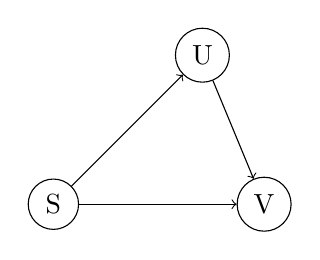
\begin{tikzpicture}[node distance=20mm, main/.style = {draw, circle}]
                % Nodes
                \node[main] (S) {S};
                \node[main] (U) [above right=of S] {U};
                \node[main] (V) [right=of S] {V};
                
                % Edges with weights 
                \draw[->] (S) -- (U);
                \draw[->] (S) -- (V);
                \draw[->] (U) -- (V);
                
            \end{tikzpicture}
        \end{center}
    
    \end{frame}
    
    
    \begin{frame}{Initial value for d}
        \textbf{Initial values:}   
        
        To assign initial values, we start with the simplest possible assumption:  
        \[
        \textcolor{red}{d[s] = 0} \quad \text{(The source reaches itself at zero cost)}
        \]
        \[
        \textcolor{red}{d[x] = \infty} \quad \text{(for all other nodes, unknown distance)}
        % \textbf{\textcolor{red}{d[x] = \infty}} \quad \text{for all other nodes (unknown distance)}
        \]   
        
    \end{frame}
    
    
    
    \begin{frame}{Value assignment for d}
        \begin{center}
            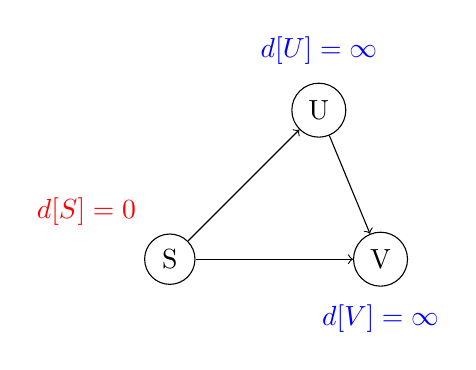
\begin{tikzpicture}[node distance=20mm, main/.style = {draw, circle}]
                % Nodes
                \node[main] (S) {S};
                \node[main] (U) [above right=of S] {U};
                \node[main] (V) [right=of S] {V};
                
                % Edges with weights
                \draw[->] (S) -- (U);
                \draw[->] (S) -- (V);
                \draw[->] (U) -- (V);
    
                % Node labels for d values
                \node[above left=3pt of S] {\textcolor{red}{$d[S] = 0$}};
                \node[above=3pt of U] {\textcolor{blue}{$d[U] = \infty$}};
                \node[below=3pt of V] {\textcolor{blue}{$d[V] = \infty$}};
                
            \end{tikzpicture}
        \end{center}
        Later, we refine these values using \textbf{edge relaxation}.
    \end{frame}
        
    \begin{frame}{Relaxing of an edge}
        \begin{center}
            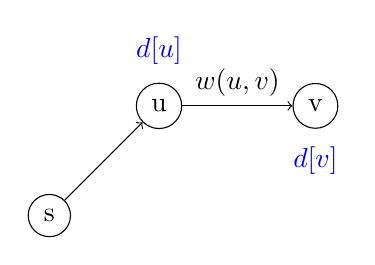
\begin{tikzpicture}[node distance=14mm, main/.style = {draw, circle}]
                % Nodes
                \node[main] (S) {s};
                \node[main] (U) [above right=of S] {u};
                \node[main] (V) [right=of U] {v};
                
                % Edges with weights
                \draw[->] (S) -- (U);
                \draw[->] (U) -- node[midway, above] {$w(u,v)$} (V);
    
                % Node labels for d values 
                \node[above=3pt of U] {\textcolor{blue}{$d[u]$}};
                \node[below=3pt of V] {\textcolor{blue}{$d[v]$}};
                
            \end{tikzpicture}
        \end{center}
        
        Given a directed weighted graph with an edge \( (u, v) \) and weight \( w(u,v) \), the relaxation step checks if:
        \[
        d[v] > d[u] + w(u,v)
        \]  
        If this condition is \textbf{\textcolor{blue}{True}}, we update:
        \[
        d[v] = d[u] + w(u,v)
        \]
    \end{frame}
    

    \begin{frame}{Example walkthrough}
        \textbf{Initial State:}
        % Initial State
        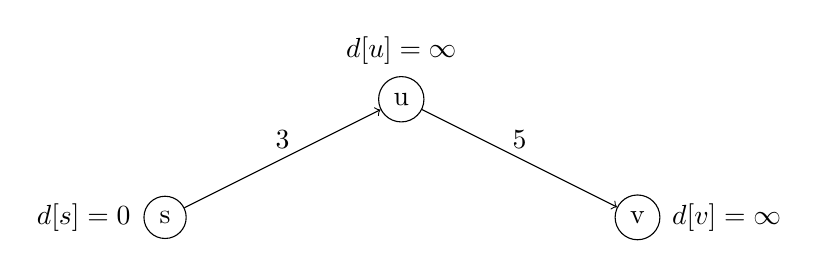
\begin{tikzpicture}[node distance=11mm, main/.style = {draw, circle}]  
            
            \node[main] (S) at (0,0) {s};
            \node[main] (U) at (3,1.5) {u};
            \node[main] (V) at (6,0) {v};
        
            \draw[->] (S) -- (U) node[midway, above] {3};
            \draw[->] (U) -- (V) node[midway, above] {5};
        
            % Distance Labels (shifted slightly outside)
            \node[left= 9pt] at (S) {$d[s] = 0$}     ; 
            \node[above=9pt] at (U) {$d[u] = \infty$}; 
            \node[right=9pt] at (V) {$d[v] = \infty$};
            
        \end{tikzpicture}
    
    \end{frame}

    \begin{frame}{Update d[u]}
        \textbf{Relaxing Edge: S → U}
        % Initial State
        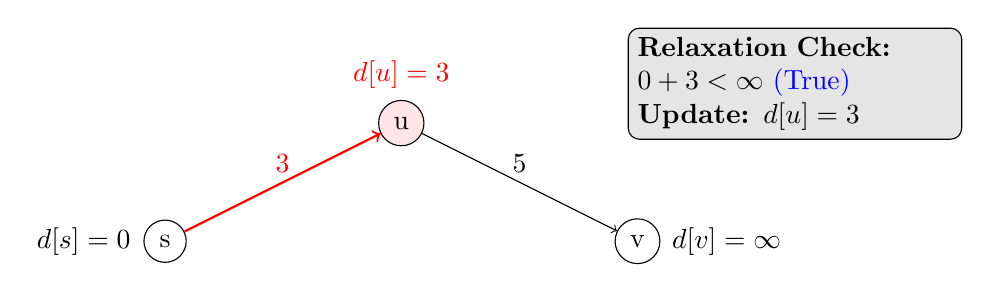
\begin{tikzpicture}[node distance=13mm, main/.style = {draw, circle}]
            
            \node[main] (S) at (0,0) {s};
            \node[main,fill=red!10] (U) at (3,1.5) {u};
            \node[main] (V) at (6,0) {v};
        
            \draw[->, thick, red] (S) -- (U) node[midway, above] {3};
            \draw[->] (U) -- (V) node[midway, above] {5};
        
            % Distance Labels (shifted slightly outside)
            \node[left= 9pt] at (S) {$d[s] = 0$}     ; 
            \node[above=9pt, text=red] at (U) {$d[u] = 3$}; 
            \node[right=9pt] at (V) {$d[v] = \infty$};

            % Relaxation Condition Box
            \node[draw, fill=gray!20, rounded corners, text width=4cm] at (8, 2) {
                \textbf{Relaxation Check:} \\
                $  0 + 3 < \infty$ \textcolor{blue}{(True)} \\
                \textbf{Update:} \textbf{$d[u] = 3$}
            };
            
        \end{tikzpicture}
    
    \end{frame}

    \begin{frame}{Update d[v]}
        \textbf{Relaxing Edge: U → V}
        
        % Initial State
        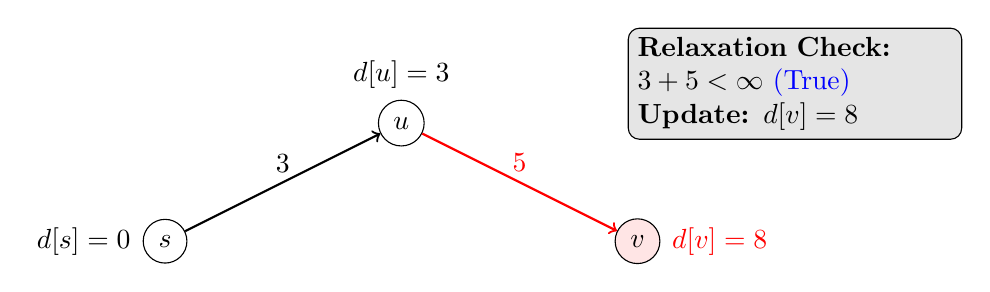
\begin{tikzpicture}[node distance=13mm, main/.style = {draw, circle}]
        
            \node[main] (s) at (0,0) {$s$};
            \node[main] (u) at (3,1.5) {$u$};
            \node[main, fill=red!10] (v) at (6,0) {$v$};
        
            \draw[->, thick] (s) -- (u) node[midway, above] {3};
            \draw[->, thick, red] (u) -- (v) node[midway, above] {5};
        
            % Distance Labels (shifted slightly outside)
            \node[left=9.pt] at (s) {$d[s] = 0$};
            \node[above=9.pt] at (u) {$d[u] = 3$};
            \node[right=9.pt, text=red] at (v) {$d[v] = 8$};
        
            % Relaxation Condition Box
            \node[draw, fill=gray!20, rounded corners, text width=4cm] at (8, 2) {
                \textbf{Relaxation Check:} \\
                % If $d[u] + w(u,v) < d[v]$ \\
                $ 3 + 5 < \infty$ \textcolor{blue}{(True)} \\
                \textbf{Update:} \textbf{$d[v] = 8$}
            };
        
        \end{tikzpicture}
    \end{frame}
    
    % ===== Properties of Shortest Paths =====
    \begin{frame}{Properties of Shortest Paths}
        \textbf{Key properties:}
        \begin{itemize}
            \item Optimal Substructure Property
            \item Edge Relaxation 
            \item Handling Non-Reachable Nodes
            \item Convergence to True Shortest Path
        \end{itemize}
    \end{frame}
    
    \begin{frame}{Optimal Substructure Property}
        The \textbf{shortest path} from S to T is:
        \begin{center}
            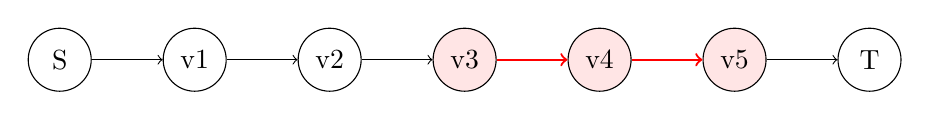
\begin{tikzpicture}[node distance=9mm, main/.style={draw, circle, minimum size=8mm}]
                \node[main] (S) {S};
                \node[main] (v1) [right=of S] {v1};
                \node[main] (v2) [right=of v1] {v2};
                \node[main,fill=red!10] (v3) [right=of v2] {v3};
                \node[main,fill=red!10] (v4) [right=of v3] {v4};
                \node[main,fill=red!10] (v5) [right=of v4] {v5};
                \node[main] (T) [right=of v5] {T};
                
                % Main path
                \draw[->] (S) -- (v1);
                \draw[->] (v1) -- (v2);
                \draw[->] (v2) -- (v3);
                \draw[->, thick, red] (v3) -- (v4);
                \draw[->, thick, red] (v4) -- (v5);
                \draw[->] (v5) -- (T);
            \end{tikzpicture}
        \end{center}
    
        What can you say about path from $\textbf{v3}$ to $\textbf{v5}$?    
    
    \end{frame}
    
    \begin{frame}{EXAMPLE}
        Since the given graph is the \textbf{shortest path} from $S$ to $T$, then the shortest path from $\textbf{v3}$ to $\textbf{v5}$ is:
     \begin{center}
            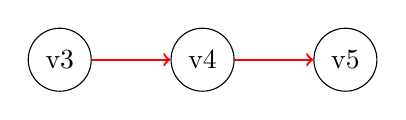
\begin{tikzpicture}[node distance=10mm, main/.style={draw, circle, minimum size=8mm}]
                \node[main] (v3) {v3};
                \node[main] (v4) [right=of v3] {v4};
                \node[main] (v5) [right=of v4] {v5};
                
                % Main path
                \draw[->, thick, red] (v3) -- (v4);
                \draw[->, thick, red] (v4) -- (v5);
            \end{tikzpicture}
        \end{center}
        % Then it must also be the shortest path from $v3$ to $v5$
    
        All \textbf{sub-paths} of a shortest path are themselves \textbf{shortest paths}!\\
          \vspace{3mm}
        \textbf{Notation:} \boldsymbol{\delta}\textbf{(s, v)} \text{ represent the shortest path from s to v}
            
    \end{frame}
    
    \begin{frame}{Edge Relaxation Mechanism}
        \textbf{Purpose:} Refine distance estimates \( d[v] \) until they match the true shortest path \( \delta(s, v) \).  
        
        \begin{columns}
            \column{0.5\textwidth}
            \centering
            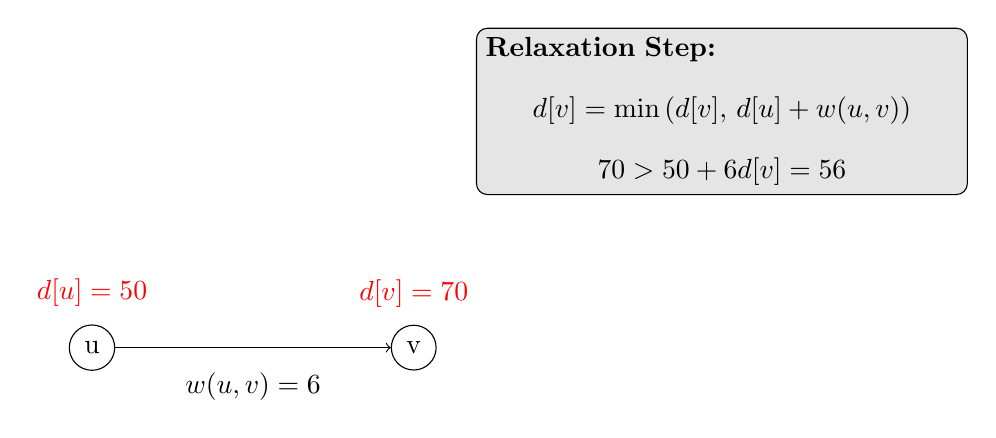
\begin{tikzpicture}[node distance=35mm, main/.style={draw, circle}]
            
                \node[main] (u) {u};
                \node[main] (v) [right=of u] {v};
                \draw[->] (u) -- node[midway, below=2mm] {$w(u,v)=6$} (v);
                
                \node[left ,above=1mm of u,text=red] {$d[u] = 50$};
                \node[right, above=1mm of v,text=red] {$d[v] = 70$};
    
                % Relaxation Condition Box
                \node[draw, fill=gray!20, rounded corners, text width=6cm]  at (8, 3) {
                    \textbf{Relaxation Step:}
                    \[
                    d[v] = \min\left(d[v],\, d[u] + w(u,v)\right)
                    \]
                    \[
                    70 > 50 + 6 \implies d[v] = 56
                    \]
                    };
                
            \end{tikzpicture}
            
            \column{0.5\textwidth}
    
        \end{columns}
    
    \end{frame}
    
    \begin{frame}{Unreachable Nodes}
        \begin{center}
            \textbf{What if we have nodes we cannot reach?}\\
            % \vspace{1. cm}
            \textbf{How does it affect our path?}
        \end{center}
    \end{frame}

    \begin{frame}{Example Graph}

        \begin{columns}
            \column{0.5\textwidth}
            \centering
            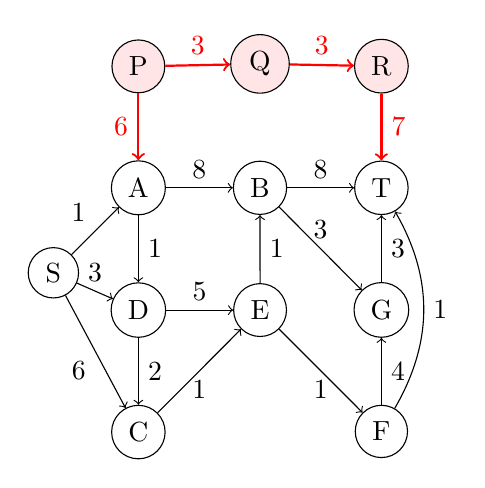
\begin{tikzpicture}[node distance=8.5mm, main/.style = {draw, circle}] 
                % Nodes
                \node[main] (S) {S};
                \node[main] (A) [above right=of S] {A};
                \node[main] (B) [right=of A] {B};
                \node[main] (D) [below=of A] {D};
                \node[main] (C) [below=of D] {C};
                \node[main] (E) [right=of D] {E};
                \node[main] (T) [right=of B] {T};
                \node[main] (G) [below =of T] {G};
                \node[main] (F) [below =of G] {F};
                \node[main,fill=red!10] (P) [above=of A] {P};
                \node[main,fill=red!10] (Q) [above=of B] {Q};
                \node[main,fill=red!10] (R) [above=of T] {R};
            
                % Edges with weights
                \draw[->] (S) --  node[midway, above left] {1} (A);
                \draw[->] (S) --  node[midway, above] {3} (D);
                \draw[->] (S) --  node[midway, below left] {6} (C);
                \draw[->] (A) --  node[midway, above] {8} (B);
                \draw[->] (A) --  node[midway, right] {1} (D);
                \draw[->] (D) --  node[midway, above] {5} (E);
                \draw[->] (D) --  node[midway, right] {2} (C);
                \draw[->] (C) --  node[midway, below] {1} (E);
                \draw[->] (B) --  node[midway, above] {8} (T);
                \draw[->] (B) --  node[midway, above] {3} (G);
                \draw[->] (E) --  node[midway, below] {1} (F);
                \draw[->] (E) --  node[midway, right] {1} (B);
                \draw[->] (F) --  node[midway, right] {4} (G);
                \draw[->] (G) --  node[midway, right] {3} (T);
                \draw[->, thick, red] (P) --  node[left] {6} (A);
                \draw[->, thick, red] (P) --  node[midway, above] {3} (Q);
                \draw[->, thick, red] (Q) --  node[midway, above] {3} (R);
                \draw[->, thick, red] (R) --  node[midway, right] {7} (T);
                
                % Curved Edge from F to T
                \draw[->, bend right=30] (F) to node[midway, right] {1} (T);
            \end{tikzpicture}
            
            \column{0.5\textwidth}
            
            If node \( V \) is unreachable from \( S \), then:
            \[
            \textcolor{red}{\boldsymbol{\delta}(s, v) = \boldsymbol{\infty}}
            \]
            \\
            \\ Node \( P \) can't be reached from S. hence, no updates during relaxation. \\

            \[
            \textcolor{red}{\boldsymbol{\delta}(S, P) = \boldsymbol{\infty}}
            \]

            \( \delta(S,P) \) remains the same.
        \end{columns}
    \end{frame}

    \begin{frame}{Perfect Estimate}
        \textbf{When do we have a perfect estimate?}
        
        \begin{itemize}
            \item When $d[u] = \delta(s,u)$, we have a perfect estimate for $u$
            \item Once perfect, the estimate never changes
            \item Estimates can either stay the same or decrease
        \end{itemize}
        
        \begin{center}
            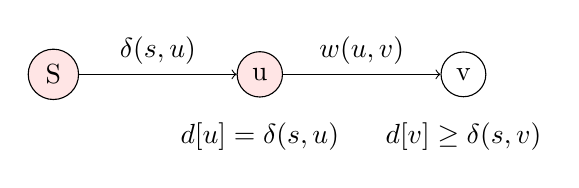
\begin{tikzpicture}[node distance=20mm, main/.style = {draw, circle}]
                \node[main, fill=red!10] (s) {S};
                \node[main, fill=red!10] (u) [right=of s] {u};
                \node[main] (v) [right=of u] {v};
                
                \draw[->] (s) -- node[above] {$\delta(s,u)$} (u);
                \draw[->] (u) -- node[above] {$w(u,v)$} (v);
                
                \node[below=2mm of u] {$d[u] = \delta(s,u)$};
                \node[below=2mm of v] {$d[v] \geq \delta(s,v)$};
            \end{tikzpicture}
        \end{center}
    \end{frame}

    \begin{frame}{Convergence to True Values}
        If we relax all the edges in the correct order we get the shortest path
          \begin{center}
                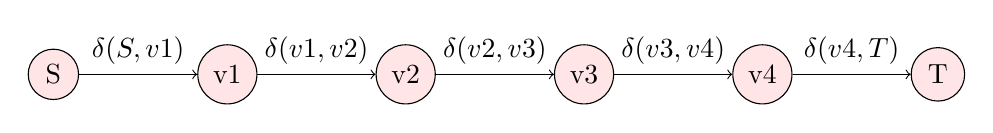
\begin{tikzpicture}[node distance=15mm, main/.style = {draw, circle}]
                
                    \node[main, fill=red!10] (S) {S};
                    \node[main, fill=red!10] (v1) [right=of S] {v1};
                    \node[main, fill=red!10] (v2) [right=of v1] {v2};
                    \node[main, fill=red!10] (v3) [right=of v2] {v3};
                    \node[main, fill=red!10] (v4) [right=of v3] {v4};
                    \node[main, fill=red!10] (T) [right=of v4] {T};
                    
                    \draw[->] (S) --node[above] {$\delta(S,v1)$} (v1);
                    \draw[->] (v1) --node[above] {$\delta(v1,v2)$} (v2);
                    \draw[->] (v2) --node[above] {$\delta(v2,v3)$} (v3); 
                    \draw[->] (v3) --node[above] {$\delta(v3,v4)$} (v4);
                    \draw[->] (v4) --node[above] {$\delta(v4,T)$} (T);
                    
                \end{tikzpicture}
            \end{center}

    \begin{itemize}
        \item \textbf{Relax (S,v1):}
              The shortest path from $S$ to v1 is updated.
        \item \textbf{Relax (v1,v2):}
              Now that we know $d[v1]$, we update $d[v2]$.
        \item \textbf{Relax (v2,v3):}
              Using $d[v2]$, we get a better estimate for $d[v3]$.
        \item Continue this process... 
              \textbf{Each step updates the shortest known distance for the next node.}
    \end{itemize}

    \vspace{0.3cm}

    \textbf{Final result:}  
    After sufficient relaxations, we get the shortest path:
    \[
    \textcolor{red}{\boldsymbol{d[v] = \delta(S, T).}}
    \]
         
    \end{frame}

    \begin{frame} {sufficient relaxes}
        \textbf{When will we have sufficient relaxes} \\
        \begin{itemize}
            \item A shortest path has at most \( V - 1 \) edges.
            \item Bellman-Ford relaxes all edges up to \( V - 1 \) times.
            \item After \( V - 1 \) relaxations, all shortest paths are computed.
        \end{itemize}

    \end{frame}
    

    \begin{frame}{Algorithm Overview}

    
        \textbf{Bellman's approach:}\\
       \begin{algorithm}
            \vspace{3mm}
            \begin{algorithmic}
                \hspace{1cm}\For{for $i = 1$ to $V-1$} 
                    \ForAll{edges $(u, v)$ in $G$}
                    \\
                       \hspace{1.5cm} \State Relax every edge $(u, v)$
                    \EndFor
                \EndFor
        \end{algorithmic}
    \end{algorithm}\\
    
        \vspace{1cm}
        \textbf{Why $V-1$ iterations?}
        \begin{itemize}
            \item Longest possible path without cycles has $V-1$ edges
            \item Ensures relaxation propagates through the entire graph
        \end{itemize}
    \end{frame}
    
    \begin{frame}{Special Case: Directed Acyclic Graphs (DAG)}
        \textbf{For DAGs:}
        \begin{itemize}
            \item we assume that there are no negative edges
            \item Perform topological sort ($O(V+E)$)
            \item Process nodes in topological order
            \item Relax all outgoing edges from each node
        \end{itemize}
        
        \textbf{Complexity:} $O(V + E)$ 
        
        \begin{center}
            \begin{tikzpicture}[node distance=15mm, main/.style = {draw, circle}]
                \node[main] (1) {1};
                \node[main] (2) [right=of 1] {2};
                \node[main] (3) [right=of 2] {3};
                \node[main] (4) [right=of 3] {4};
                
                \draw[->] (1) -- (2);
                \draw[->] (2) -- (3);
                \draw[->, bend right=30] (1) to node[midway, right] {} (3) 
                \draw[->, bend right=30, ] (2) to node[midway, right] {} (4)
                
                \draw[->] (3) -- (4);
                
                \node[above=2mm of 1] {Topological Order};
            \end{tikzpicture}
        \end{center}
    \end{frame}
    \begin{frame}{example walk through}
    \textbf{First iteration}
    
    \text{We relax all the edges going from \textbf{1}}\\
       \begin{itemize}
           \item relax(1,2)
           \item relax(1,3)
       \end{itemize}
    \begin{center}
            \begin{tikzpicture}[node distance=15mm, main/.style = {draw, circle}]
                \node[main,fill= red!10] (1) {1};
                \node[main] (2) [right=of 1] {2};
                \node[main] (3) [right=of 2] {3};
                \node[main] (4) [right=of 3] {4};
                
                \draw[->, thick, red] (1) to node[midway, above] {$\delta(1,2)$} (2);
                \draw[->] (2) -- (3);
                \draw[->, bend right=30, thick, red] (1) to node[midway, below] {$\delta(1,3)$} (3) 
                \draw[->, bend right=30, ] (2) to node[midway, right] {} (4)
                
                \draw[->] (3) -- (4);
                
                \node[above=2mm of 1] {Topological Order};
            \end{tikzpicture}
        \end{center}
    
    
        
    \end{frame}
    
    \begin{frame}{example walk through}
    \textbf{Second iteration}
    
    \text{Now we relax all the edges going from \textbf{2}}\\
       \begin{itemize}
           \item relax(2,3)
           \item relax (2,4)
        
       \end{itemize}
    \begin{center}
            \begin{tikzpicture}[node distance=15mm, main/.style = {draw, circle}]
                \node[main] (1) {1};
                \node[main,fill= red!10] (2) [right=of 1] {2};
                \node[main] (3) [right=of 2] {3};
                \node[main] (4) [right=of 3] {4};
                
                \draw[->] (1) to node[midway, above] {$\delta(1,2)$} (2);
                \draw[->,thick, red] (2) to node [midway,above] {$\delta(2,3)$} (3);
                \draw[->, bend right=30] (1) to node[midway, below] {$\delta(1,3)$} (3) 
                \draw[->, bend right=30,thick,red ] (2) to node[midway, below] {$\delta(2,4)$} (4)
                
                \draw[->] (3) -- (4);
                
                \node[above=2mm of 1] {Topological Order};
            \end{tikzpicture}
        \end{center}
        \end{frame}
    
    \begin{frame}{example walk through}
    \textbf{Third iteration}
    
    \text{Now we relax all the edges going from \textbf{3}}\\
       \begin{itemize}
           \item relax(3,4)
          
        
       \end{itemize}
    \begin{center}
            \begin{tikzpicture}[node distance=15mm, main/.style = {draw, circle}]
                \node[main] (1) {1};
                \node[main] (2) [right=of 1] {2};
                \node[main,fill= red!10] (3) [right=of 2] {3};
                \node[main] (4) [right=of 3] {4};
                
                \draw[->] (1) to node[midway, above] {$\delta(1,2)$} (2);
                \draw[->] (2) to node [midway,above] {$\delta(2,3)$} (3);
                \draw[->, bend right=30] (1) to node[midway, below] {$\delta(1,3)$} (3) 
                \draw[->, bend right=30 ] (2) to node[midway, below] {$\delta(2,4)$} (4)
                
                \draw[->,thick, red] (3) to node [midway, above] {$\delta(3,4)$}  (4);
                
                \node[above=2mm of 1] {Topological Order};
            \end{tikzpicture}
        \end{center}
    
    \text{After \textbf{n-1} iterations we have relaxed all the edges}
        
    \end{frame}
    
    \begin{frame}{Summary of Properties}
        \textbf{Summary:}
        \begin{itemize}
            \item \textbf{Optimal Substructure:} Shortest paths are built from shortest sub-paths.
            \item \textbf{Initialization:} \( d[s] = 0 \),\( d[v] = \infty \) for others.
            \item \textbf{Relaxation:} Iteratively improves estimates using edges.
            \item \textbf{Non-Reachable Nodes:} Remain at \( \infty \).
            \item \textbf{Convergence:} Guaranteed after \(|V| - 1\) relaxations in a graph without negative cycles.
        \end{itemize}
    \end{frame}
    
    \begin{frame}{Complexity Analysis}
        \textbf{General Case:}
        \begin{itemize}
            \item  time complexity: $O(VE)$ 
        \end{itemize}
    
        % \textcolor{red}{\textbf{What happens if thegraph is dense?} }\\
        \textbf{For dense graph:}
        \begin{itemize}
            \item time complexity: $O(V^3)$
        \end{itemize} 
    \end{frame}

    \begin{frame} {Complexity in dense graph}
        \textbf{Why $\mathbf{O(V^3)}$ for Dense Graphs?} \\
        For dense graphs: 
        \[ |E| \approx |V|^2 \]
        \[ O(VE) = O(V \cdot V^2) = O(V^3) \]
    \end{frame}

    \begin{frame} {Comparison}
        \textbf{Comparison:}
        \begin{itemize}
            \item Brute Force: $O(2^n)$ (exponential)
            \item Bellman-Ford: $O(VE)$ (linear)
            % \item DAG: $O(V+E)$ (linear)
        \end{itemize}
    \end{frame}
    

\end{document}
